\section[Results]{Results}
\label{sec:results}

\begin{frame}{Results: Real World Data}
	\begin{figure}
		\centering
		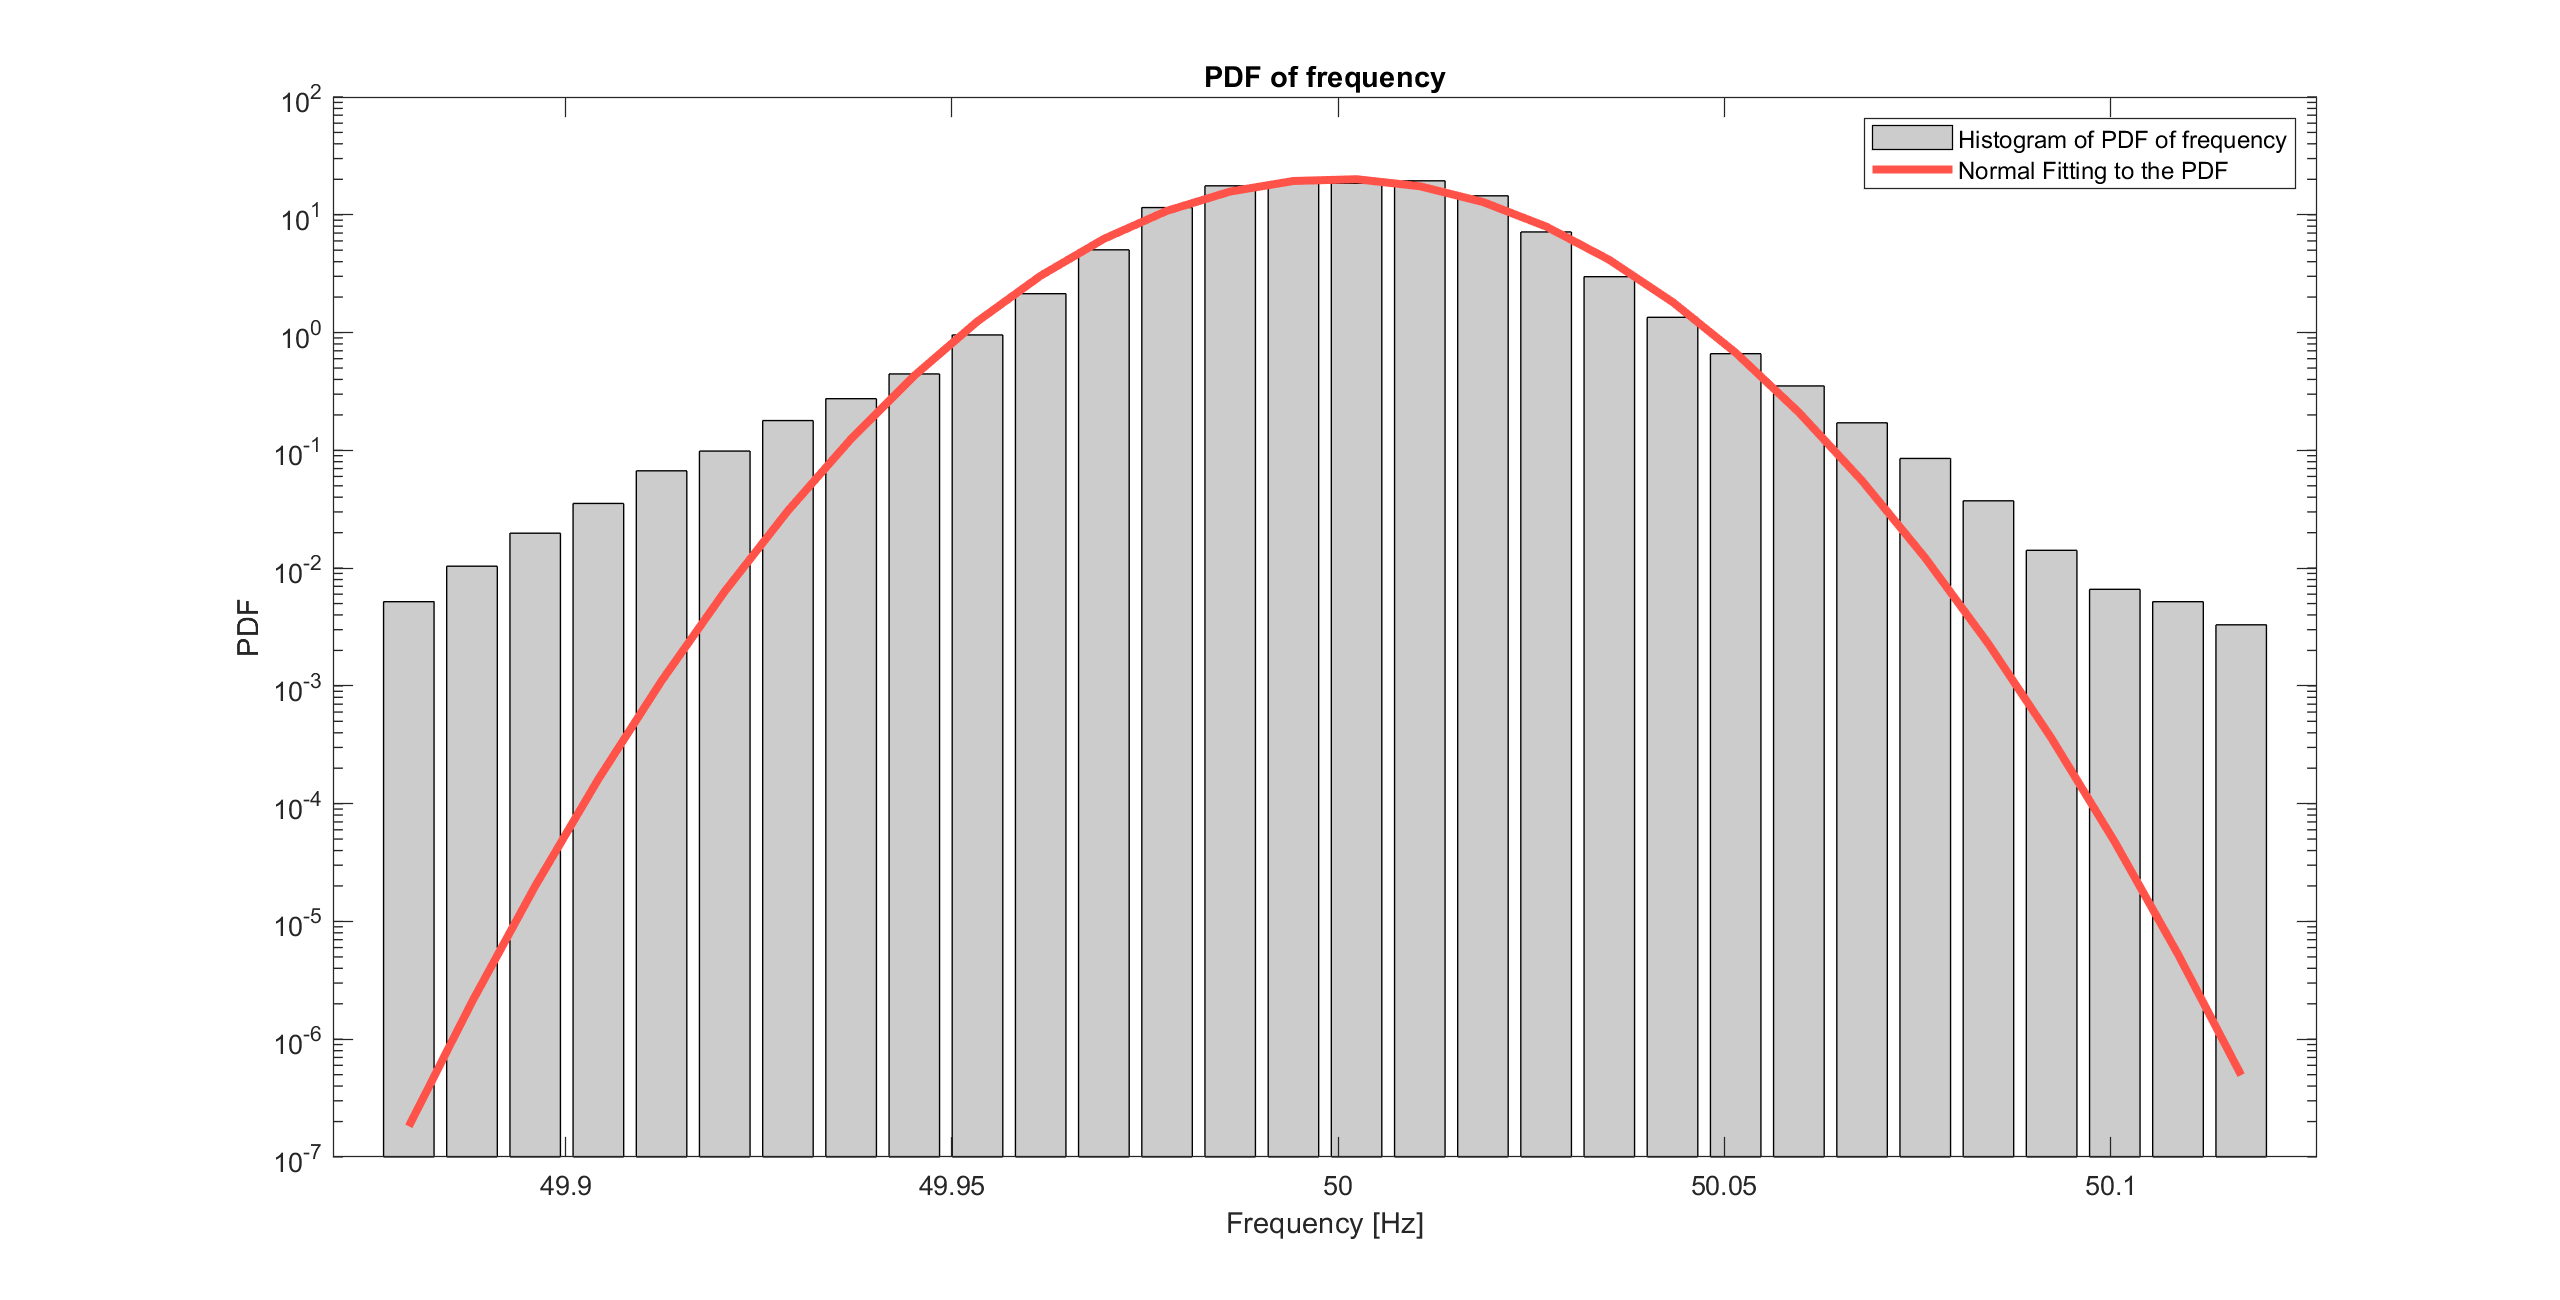
\includegraphics[scale=0.15]{../figures/pdf/pdf_frequency_rte_2019_09.png}
		\label{fig:pdf_rte2019}
		\caption{Continental European Grid frequency PDF: Heavier tails than a Gaussian Distribution.}
	\end{figure}
\end{frame}

\begin{frame}{Results: Real World Data}
	\begin{figure}
		\centering
		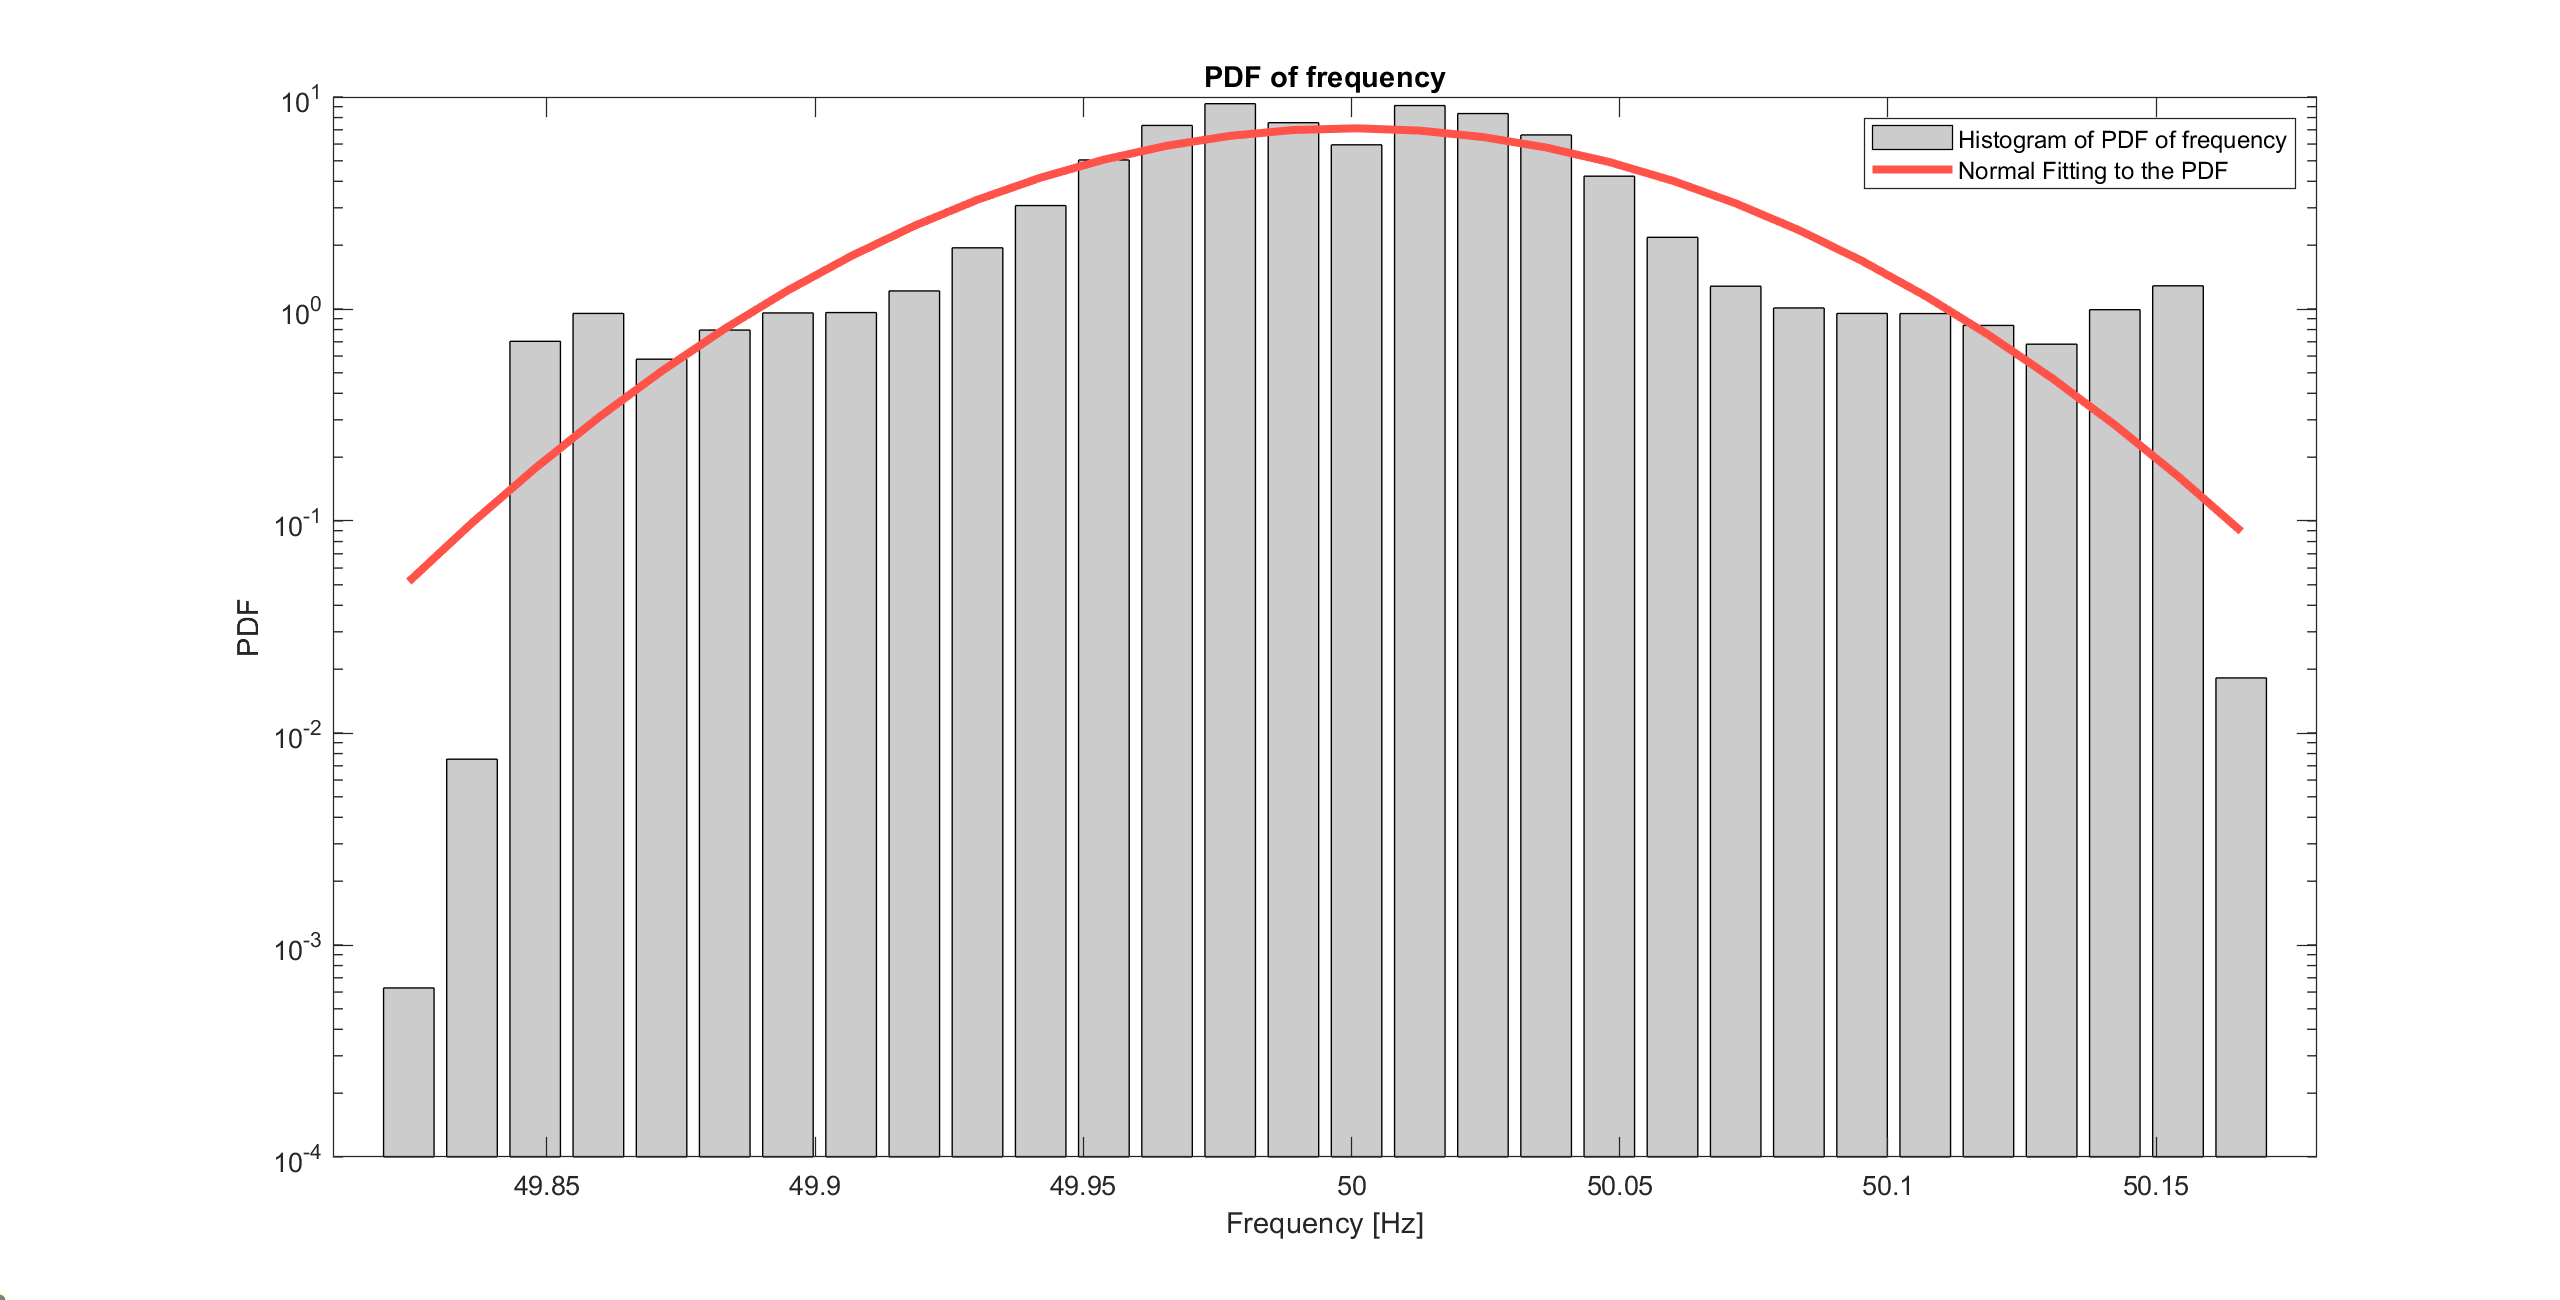
\includegraphics[scale=0.15]{../figures/pdf/pdf_frequency_spain_mallorca_2019_05_f1}
		\label{fig:pdf_spainMallorca}
		\caption{Mallorcan (an islanded Spanish grid) frequency pdf}
	\end{figure}
\end{frame}

\begin{frame}{Results: Real World Data}
	\begin{figure}
		\centering
		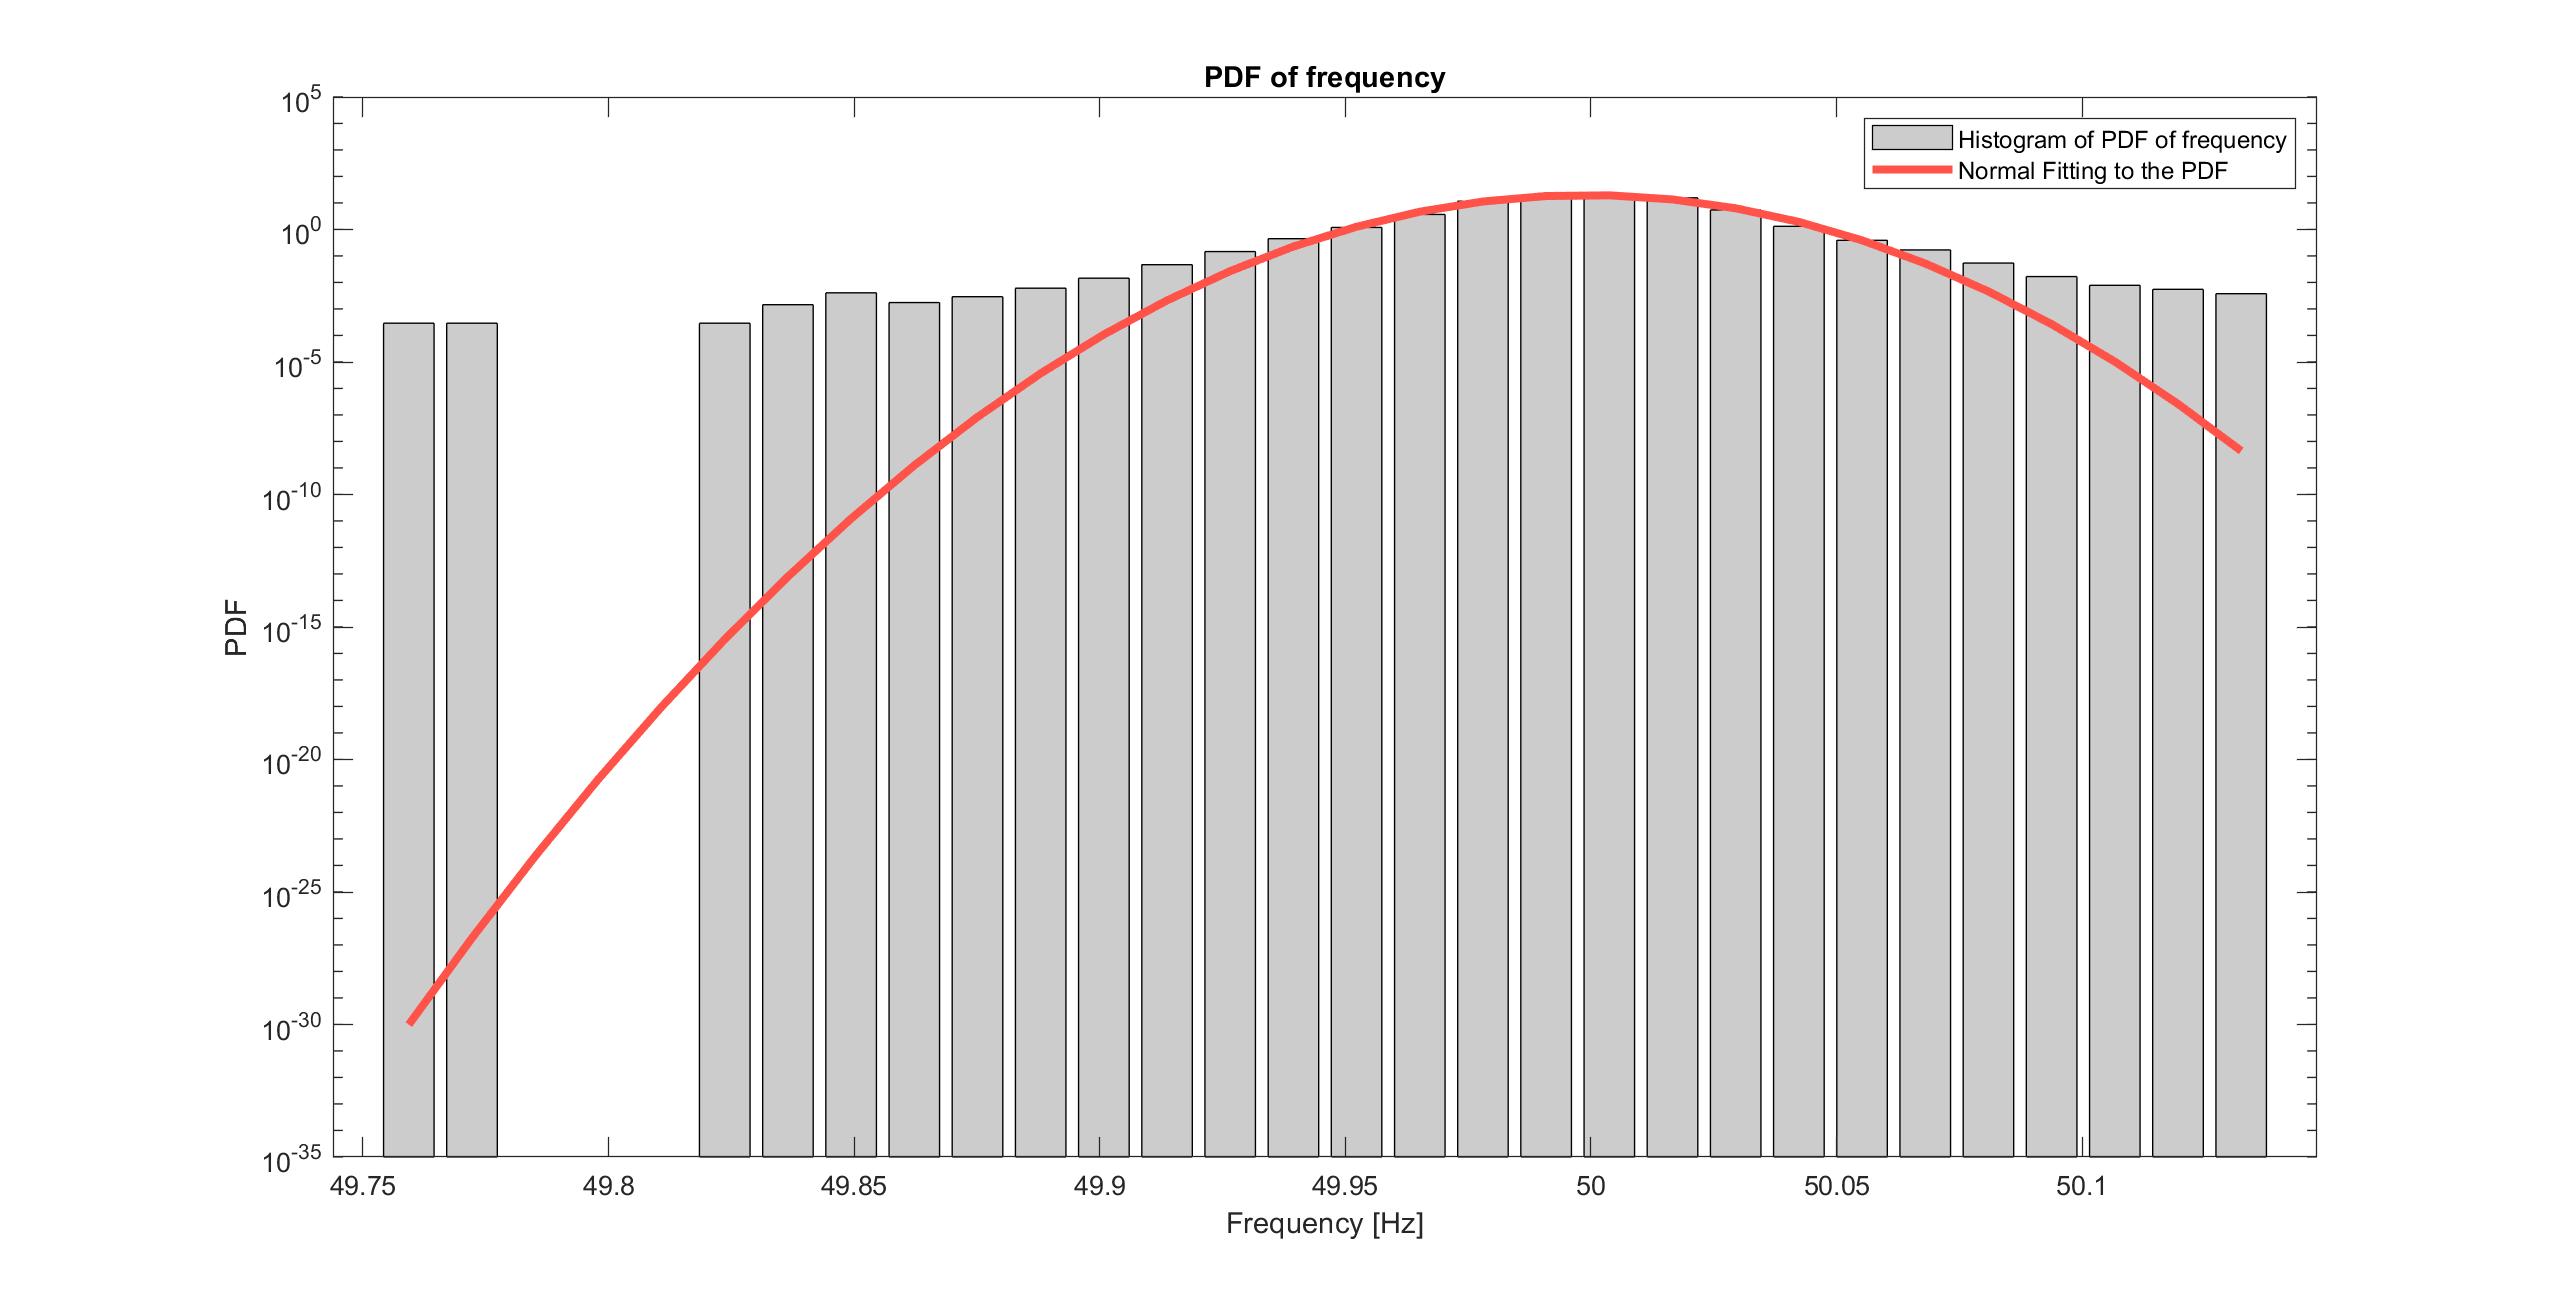
\includegraphics[scale=0.15]{../figures/pdf/pdf_frequency_rte_2021_01_blackout}
		\label{fig:pdf_rte2021blackout}
		\caption{French grid frequency pdf including a blackout}
	\end{figure}
\end{frame}

\begin{frame}{Results: Real World Data}	
	\begin{figure}[ht]
		\centering
		\resizebox{0.75\linewidth}{!}{\import{../figures/autocorr}{comparison_five_no_title.tex}}
		\caption{Autocorrelation decay of different synchronous regions.}
		\label{fig:comp5}
	\end{figure}
\end{frame}

\begin{frame}{Results: Real World Data}
	\begin{figure}
		\centering
		\import{../tables/}{inverseAutocorrelationValues}
		\label{tab:invAutocorr}
		\caption{Inverse correlation time is proportional to the damping constant of the grid.}
	\end{figure}	
\end{frame}

\begin{frame}{Results: PSSE Simulation}
	\begin{figure}
		\centering
		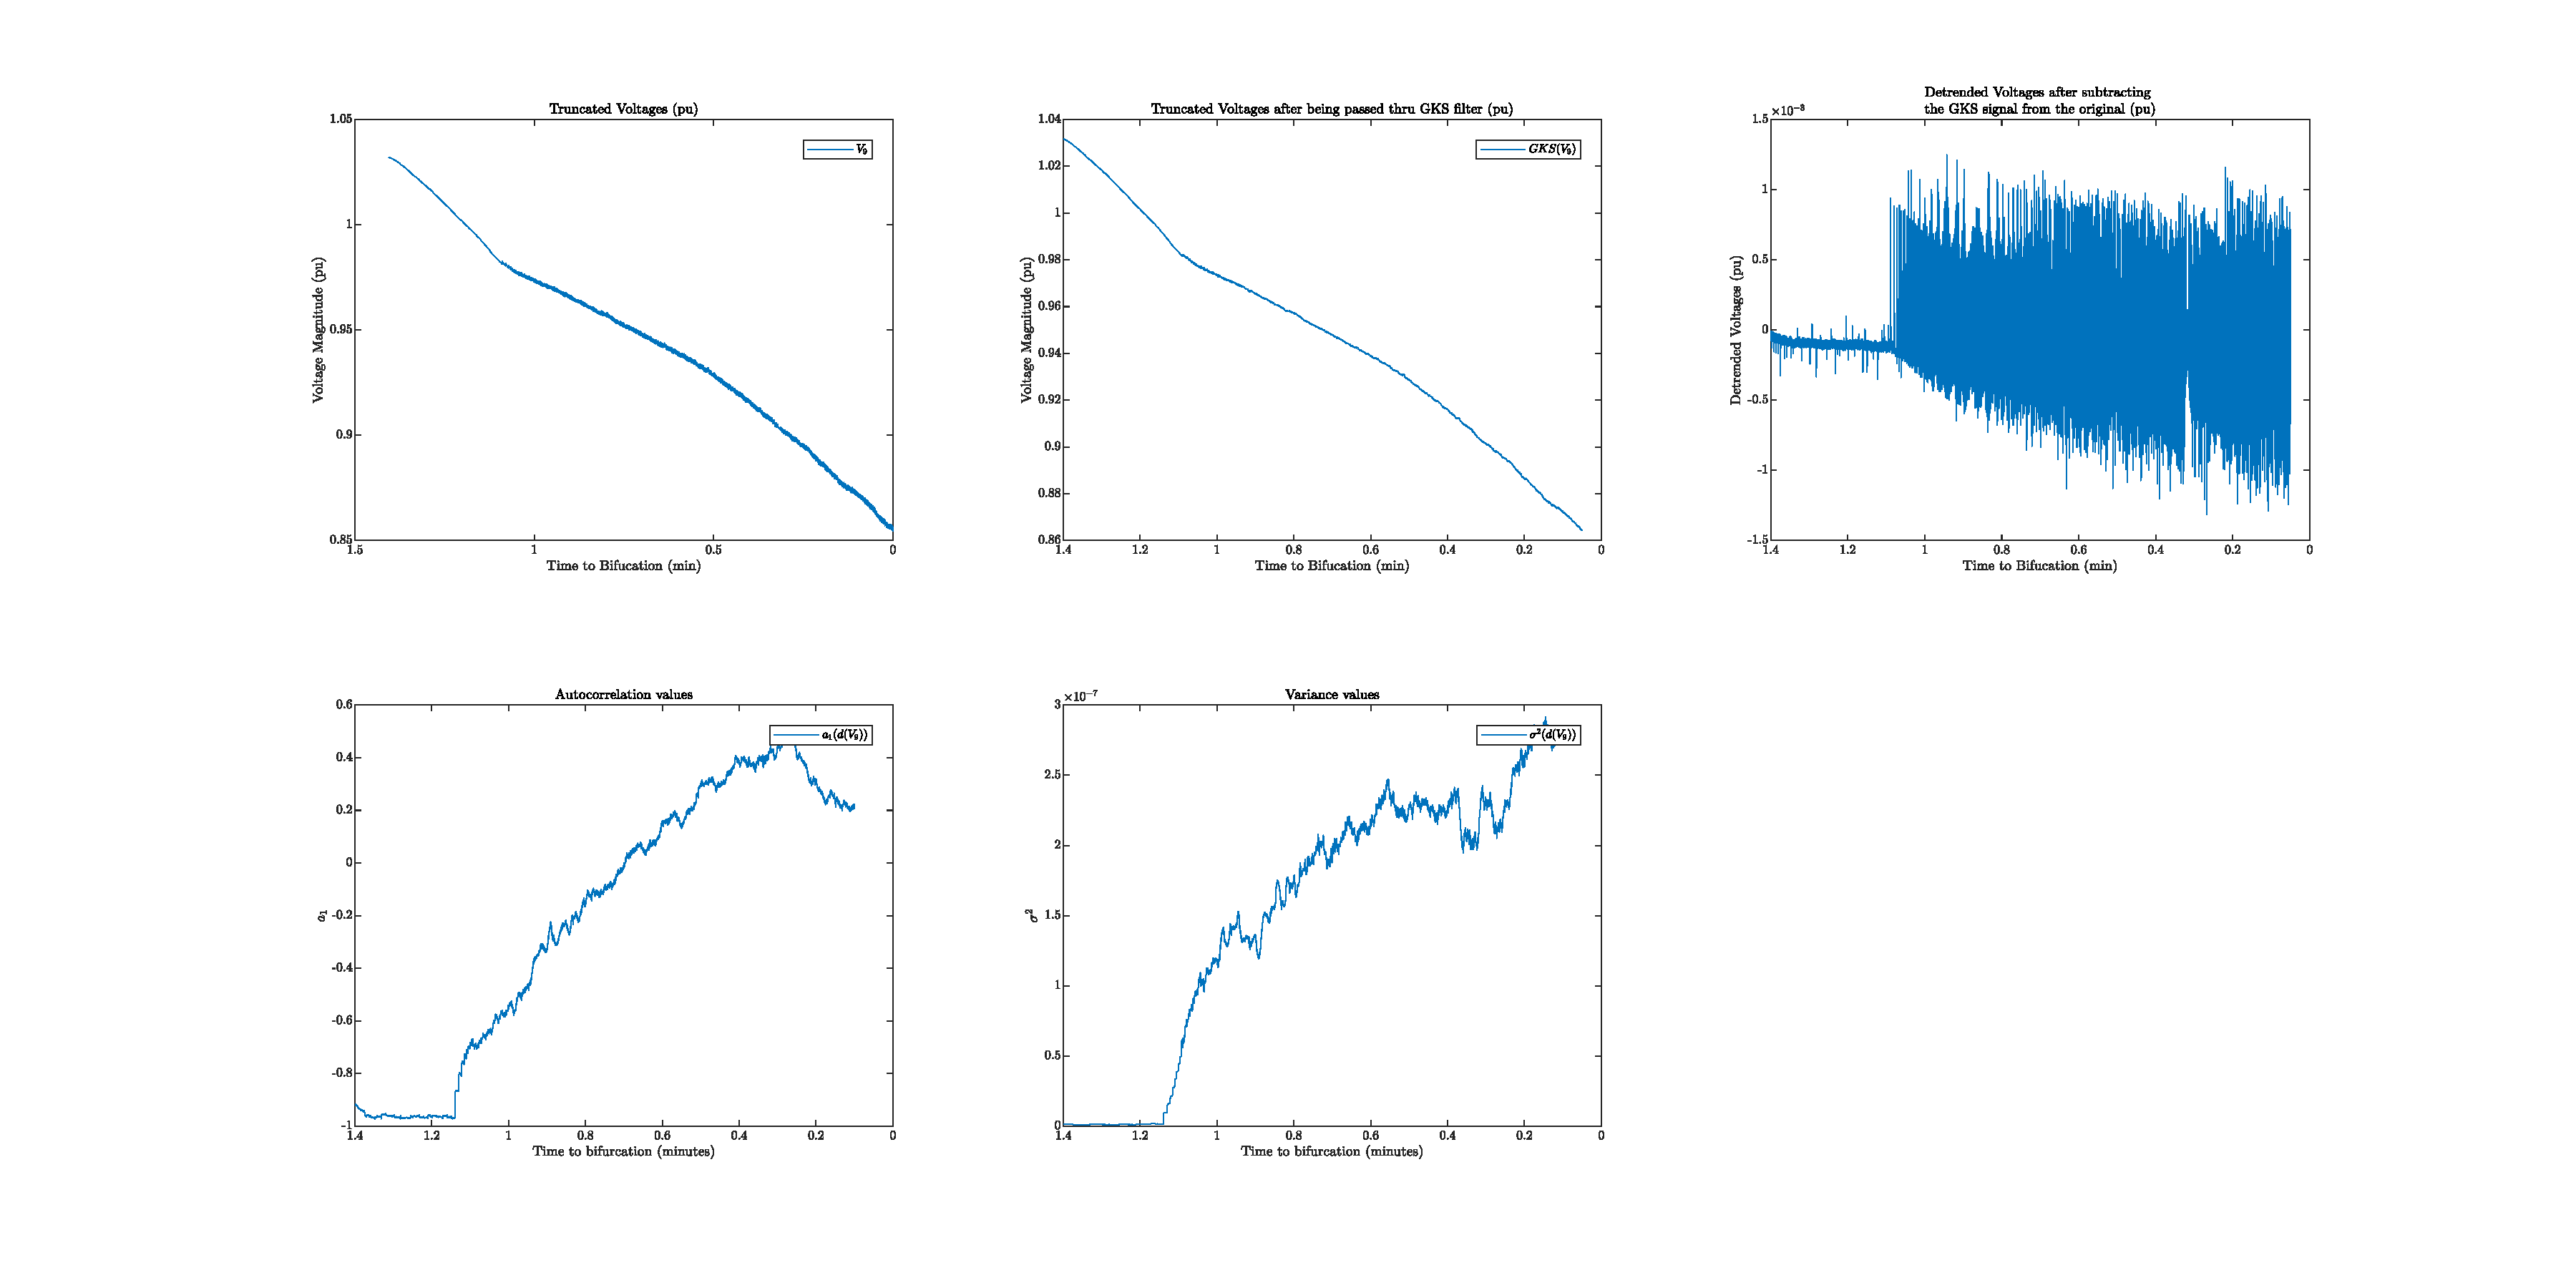
\includegraphics[scale=0.20]{../figures/pdf/_ieee9busVoltages_9_T_3_sec.pdf}
		\label{fig:pdf_9bussystem}
		\caption{Analysis of a bus voltage for the IEEE 9 Bus system vs a constant load increment.}
	\end{figure}
\end{frame}
